\subsubsection{Rancangan Detail Komponen HTTP Server}
\label{subsubsection:detail-komponen-HTTP-server}

Komponen HTTP \textit{server} berfungsi sebagai antarmuka komunikasi antara \textit{client} dan \textit{Node}. Komponen ini bertanggung jawab untuk menerima dan memproses permintaan dari \textit{client}, serta mengirimkan respons yang sesuai.

Ilustrasi struktur komponen HTTP \textit{server} dapat dilihat pada gambar \ref{fig:http-server-structure}.

% _TODO: Change image
\begin{figure}[ht]
    \centering
    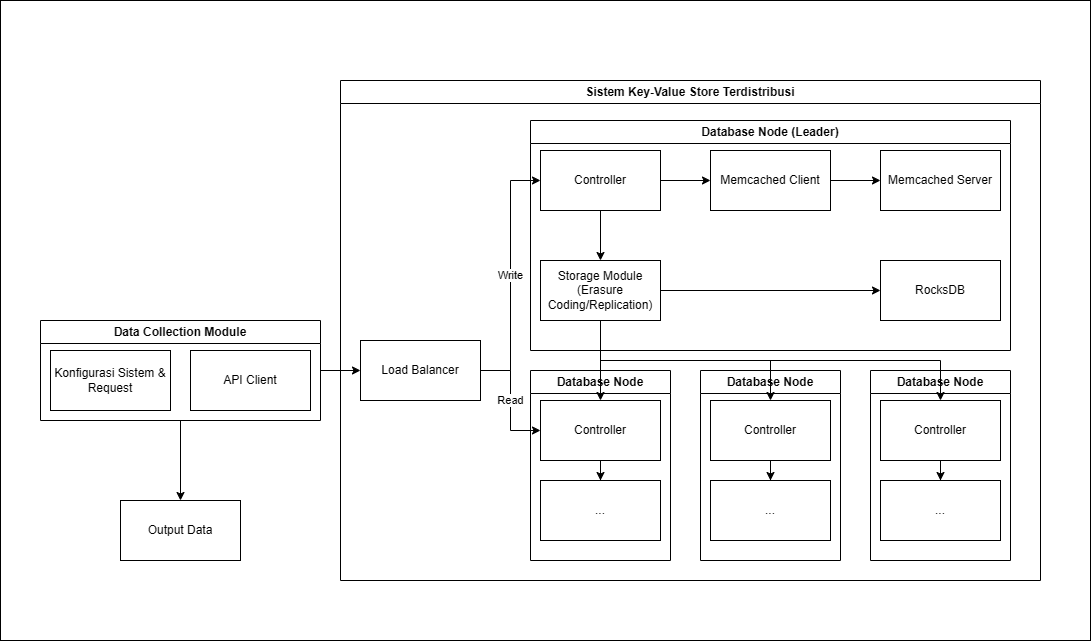
\includegraphics[width=0.95\textwidth]{resources/chapter-3/general-architecture.png}
    \caption{Struktur Komponen HTTP Server}
    \label{fig:http-server-structure}
\end{figure}
